\title{ }
\author{
        Justin Baraboo \\
         Design and Analysis of Algorithms\\
        Assignment 5\\
       }


\documentclass[12pt]{article}
\usepackage{amsmath}
\usepackage[pdftex]{graphicx}
\usepackage{listings}
\usepackage{color}

\usepackage{pgf}
\usepackage{tikz}
\usetikzlibrary{arrows,automata}
\usepackage{fancybox}


\definecolor{dkgreen}{rgb}{0,0.6,0}
\definecolor{gray}{rgb}{0.5,0.5,0.5}
\definecolor{mauve}{rgb}{0.58,0,0.82}

\lstset{frame=tb,
  language=Java,
  aboveskip=3mm,
  belowskip=3mm,
  showstringspaces=false,
  columns=flexible,
  basicstyle={\small\ttfamily},
  numbers=none,
  numberstyle=\tiny\color{gray},
  keywordstyle=\color{blue},
  commentstyle=\color{dkgreen},
  stringstyle=\color{mauve},
  breaklines=true,
  breakatwhitespace=true,
  tabsize=3
}

\begin{document}
\maketitle


\section{Problem 1}
Please prove that for a given positive number k, finding a generalized traveling salesman tour such that its total weight is less than or equal to k is an NPC problem.

\paragraph{Solution}
To show that the optimized generalized traveling salesman tour is an NPC problem we must show that it is in NP and that there exists a NPC problem that polynomially reduces to it.\\
First we will show that it is in NP by showing that a certificate can be verifed in polynomial time.  Given a certificate p and a graph with vertices V, edges E, and wanting to find a tour less than k, we construct the verifier as shown:

\begin{lstlisting}

GeneralizeSaleVer( G(V,E,k), p)
{
   Make sure all nodes in p are in V
   Make sure all nodes in V are in p at least once
   Make sure all edges in p are in E
   Make sure node starting in p is ending node in p
   Make sure the sum of weights of edges in p are less than k
   
   If yes to all, return yes. Else return no.
}

\end{lstlisting}

Now we must show that there exists an NPC problem that polynomially reduces to this problem, that is if we can solve the optimized generalized traveling salesman tour we can solve it through a polynomial transform, and thus solve any problem in NP.  We will polynomially reduce the hamiltonian cycle problem to this problem.  \\

For the hamiltonian cycle problem, for a graph G(V,E) we wish to find a cycle starting at a node s which returns to s and visits every node exactly once.  We will transform the problem in the following way: give all the edges weight $1$.  Ask the generalized traveling salesman problem to see if it can find a tour of distance less than or equal to $n$ the number of nodes in the graph.\\
To justify this is right, assume that we have a hamiltonian cycle.  Then there exists a path that visits every node exactly once and returns to the source.  Our generalized traveling salesman tour can merely follow this path and its distance will be $n$.\\
Now assume we have a generalized traveling salesman tour of distance $n$.  Then it can only visit $n$ nodes else it's distance would be greater.  Since it must visit each node at least once, it must visit them exactly once.  Thus it is also a Hamiltonian cycle of the original graph.\\
Thus Ham Cycle $ \leq_P$ Generalized Traveling Salesman.\\
Thus Generalized Traveling Salesman $\in$ NPC.


\section{Problem 2}
Prove that finding two disjoint paths whose distances are both less than $k$ is NP-Hard.

\paragraph{Solution}

To prove something is NP-Hard we only need to find an problem in NPC which is polynomially reducible to it.  We will reduce the set partition problem to this problem.  That is if you have a set of $n$ numbers, the set partition problem decides if the set can be partitioned into two disjoint subsets whose union forms he original set, such that the sum of each subset is equal.\\

So given $n$ numbers, we construct a graph, in polynomial time, as shown below:

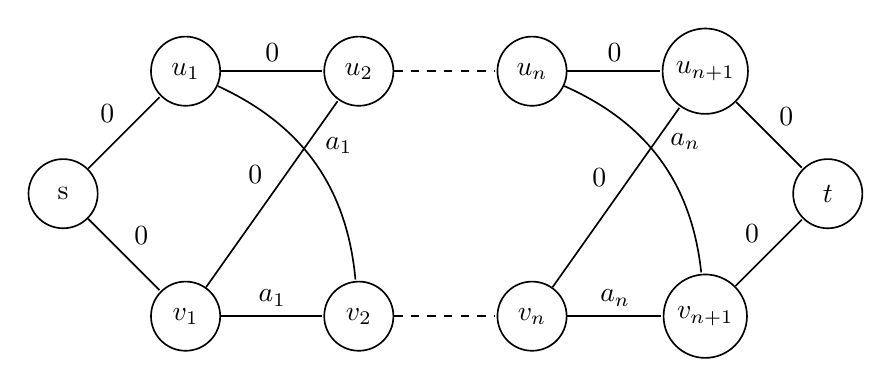
\begin{tikzpicture}[-,>=stealth',shorten >=.5pt,auto,node distance=2.2cm,
                    semithick]
%  \tikzstyle{every state}=[fill=white,draw=none,text=black]


 \node [state]      (S) {s};
 \node [state]      (u1)[above right of=S] {$u_1$};
 \node [state]      (v1) [below right of=S]{$v_1$};
 \node [state]      (u2)[right of = u1] {$u_2$};
 \node [state]      (v2)[right of =v1] {$v_2$};

\node [state]      (un)[right of = u2] {$u_n$};
 \node [state]      (vn)[right of =v2] {$v_n$};
\node [state]      (ul)[right of = un] {$u_{n+1}$};
 \node [state]      (vl)[right of =vn] {$v_{n+1}$};
 \node [state]      (t)[below right of =ul] {$t$};

 \path (S) edge         node {0} (u1)
                edge         node{0}  (v1)

         (u1) edge        node{0} (u2)
         (u1) edge       [bend left] node{$a_1$} (v2)

         (v1) edge        node{0} (u2)
         (v1) edge        node{$a_1$} (v2)

         (u2) edge       [dashed] node{} (un)
         (v2) edge       [dashed] node{} (vn)

         (un) edge        node{0} (ul)
         (un) edge     [bend left] node{$a_n$} (vl)

         (vn) edge     node{0} (ul)
         (vn) edge        node{$a_n$} (vl)

         (ul) edge        node{0} (t)
         (vl) edge        node{0} (t)


;
  \end{tikzpicture}

We then ask if we can find two disjoint paths such that distance of both paths is less than $\frac{m}{2}$ where $m$ is the sum of all the numbers in the set $n$.  If such two paths exist, then the set can be paritioned into two subsets such that they are equal.\\
To explain this, notice that at each $u_i$ and $v_i$ both paths must each either switch tracks or stay on the same track  (otherwise they wouldn't be disjoint).  So if they stay, bottom track path gets $a_i$, but if they swap then top track gets $a_i$'s edge, but, importantly, they cannot pick the same edge (which represents a number in the set).  So if one path keeps taking $0$ the other path must accumulate all the elements in the set and thus be greater than $\frac{m}{2}$.  So if we assume that our set can be partitioned, then the two paths must exist as two sets of numbers exist such that their total is $\frac{m}{2}$ and our path can choose those edges.  If we assume that we can find those paths in our graph, then our set can be partitioned as the paths essentially picks the edges, which correspond to numbers, which need to be in each set.  

\section{Problem 3}
	Suppose we need to ship coal from a coal mine to two cities, A and B, by trucks. There are $n > 3$ trucks are available. Their capacities are $c_1, c_2,$ ...  $,c_n$ (tons). We wish to divide the trucks into two groups which are responsible to ship the coal to city A and city B respectively. Because the distance from the mine to city A is longer than the distance to city B, we will collect 60 dollars from city A for every ton of coal we ship to this city and collect 30 dollars from city B for each ton of coal. Suppose every truck must be fully loaded and belong to one of the groups. Now, the question is: Can we divide the trucks into two groups such that we will collect exactly equal amount of money from the two cities. Please prove that this decision problem is NP-hard.

\paragraph{Solution}
To prove something is NP-Hard we only need to find an problem in NPC which is polynomially reducible to it.  We will reduce the set partition problem to this problem.  That is if you have a set of $n$ numbers, the set partition problem decides if the set can be partitioned into two disjoing subsets, whose union is the entire set, such that the sum of each subset is equal.\\
Note that in this problem, we are really asking if we can find a partition such that the two disjoint subsets, which together form the entire set, such that one is twice as big as the other.
\\
So to solve this problem we first  shift our numbers until they are all natural numbers and then multiply every element in our original set by $2$ (this doesn't change what our set partitioning would be if it exists as we are doing non-zero multiplication to both sides of the equation) . Let $m = \sum\limits_{x \in Set} \frac{x}{2}$, that is the sum of the entire set divided by two. We append $m + 3$ and $1.5$ to the set.\\
If we can find a partitioning of "cars" with this set, we can find a set partition in our original problem.  If we can't, then we can't.\\
To justify this, assume we have a set partitioning which we append those numbers to.  Note that if we write our coal problem as trying to find $ 2(a_i +... a_j) = (a_k + ... + a_l)$ then $m+3$ must be on the right hand side and $1.5$ must be on the left hand side.  This is because $2 * (m +3 + 1.5) > n$ so the elements cannot sum up to it.  They cannot both be on the right hand side as everything is even and $1.5$ isn't (and is a decimal) so it cannot have a counterpart.  Also $1.5$ must be on the left hand side as everything is a integer but it.  Thus $m+3$ must be on the right hand side. \\
So assume we have a set partition. Then our there will also exist a partition such that two subsets are equal to $m$.  Thus $ 2(a_i +... +a_j) + 3 = m +3 + (a_k +... + a_l)$ or that $2 m = m + m$. \\


Now assume that we can parition the cars, it will be of the form $ 2(a_i +... +a_j) + 3 = m +3 + (a_k +... + a_l)$.  If the left subset's sum is $x$ then the right subsets will be $2m -x$. Leaving: $2x = m + 2m -x \iff 3x = 3m \iff x = m$  that is each partitoning of our original sets could be $ \sum\limits_{x \in Set} \frac{x}{2}$ and moreover equal.\\
Thus Coal Problem $\in$ NP-Hard.


\section{Problem 4}
Suppose we are going to hold a conference. The conference covers m different topics. For each topic, we have a list, $T_i$, $1 \leq i \leq m$, of professors who can review papers on this topic. One professor may be able to review papers on multiple topics. An optimization problem is to select a minimum number of professors to form a program committee that can handle paper review for all topics. We assume there are a total of n professors, denoted by set $P = \{p_1, p_2, …, p_n\}$.

\paragraph{Solution}
To redefine this as a decision problem, we ask if there exists $k$ professors to cover $m$ topics.\\
To show that this is in NP, we must show that there exists a verifier for a certificate $p$, a set of professors (which can be represented as a set of topics covered). We do this below, note Parray is our array of professors and $m$ is the number of topics $1...m$: \\
\begin{lstlisting}
ProfSched( A( Parray, m), p)
     {
        Make sure all professors in p are in Parray
        Does p contain less than k professors?
        Make sure that all m topics are covered by at least one professor in p
         (iterate through each professor in p, and mark covered in a 1...m size array
           if one all 1...m are covered then good)
        Return yes if above is right, no othewise
      }

\end{lstlisting}


Finally, to show that this in NPC, we must reduce a known NPC problem to it.  We will use vertex cover.
Assume we can solve professor problem, then we must merely transform the vertex cover problem into professor problem and use it to solve.
      Each professor is merely a set of topics.      For graph G(V,E) in vertex cover, label the $m$ edges, starting at the left and going up to down.\\
      For each node, represent it as a set of edges it touches.  
      Unify each of these into a containing set, e.g: $\{ \{2,3,4\} , \{ ... \}, \{ ...\}, \{ ... \},..., \{ ... \} \}$
      These sets act as a professors for topics.
       Finding smallest number of professors to cover topics (edges) finds the smallest
     set of vertex cover.
\\
To justify this, assume we have a vertex cover with $k$ nodes.  Then we can easily find a professor set which covers $m$ topics (the vertices chosen are the professors chosen) as those nodes cover $m$ edges..
Assume that we have a professor problem that only needs $k$ professors from our transform.  Then those professors represent nodes in our graph which cover it as those professors cover $m$ topics (edges).


\end{document}